
\begin{frame}
  \frametitle{What is quality code ?}

\begin{exampleblock}{}
  {\large ``Quality is form and function. Code should work as expected when I use it.''}
%  \vskip5mm
%  \hspace*\fill{\small--- IKEA Catalog, 2017}
\end{exampleblock}
\end{frame}

\begin{frame}
   \begin{center}
   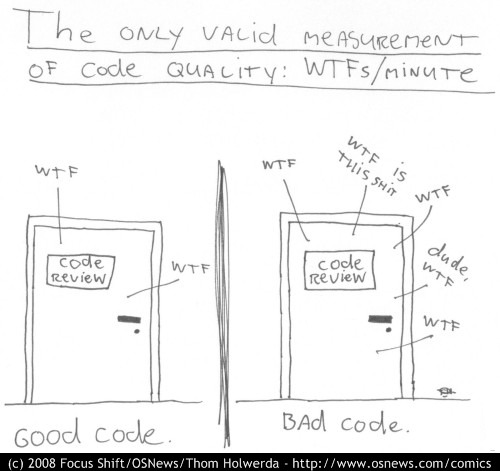
\includegraphics[width=\textwidth,height=0.8\textheight,keepaspectratio]{wtfm.jpg}
   \end{center}
\end{frame}

\begin{frame}
  \frametitle{Bad code}
  Developers think:
  \begin{itemize}
  \item No time\pause
  \item Other bad code\pause
  \item Poor design\pause
  \item Lack of skills\pause
  \item Lack of Domain knowledge\pause
  \item Don't care\pause
  \end{itemize}
\end{frame}

\begin{frame}
  \frametitle{Clean bad code}
  \begin{minipage}[t]{0.48\linewidth}
    \begin{itemize}
        \item Involves risks\pause
        \item Takes time\pause
        \item Necessary\pause
        \item Can be fun\pause
    \end{itemize}
  \end{minipage}\hfill
  \begin{minipage}[t]{0.48\linewidth}
      \begin{itemize}
          \item Version Control\pause
          \item Test Suite
      \end{itemize}
  \end{minipage}
\end{frame}


%\begin{frame}
%  \frametitle{Пример 1}
%  Качествения код е лесен за:
%  \begin{itemize}
%  \item разбиране от хора
%  \item развиване
%  \item поддръжка
%  \end{itemize}
%\end{frame}


%\begin{frame}
%  \frametitle{Пример 2: GotoBLAS}
%  Качествения код:
%  \begin{itemize}
%  \item оптимизиран до максимум
%  \item за специализиран процесор
%  \item асемблер
%  \end{itemize}
%\end{frame}


%\begin{frame}
%  \frametitle{Пример 3: Sparse Suite}
%  Качествения код:
%  \begin{itemize}
%  \item разнообразни алгоритми
%  \item високопроизводителен
%  \item минимални дефекти
%  \end{itemize}
%\end{frame}


%\begin{frame}
%  \frametitle{Sparse Suite}
%  MATLAB: $A \vec{x} = \vec{b}$ 
%  \begin{itemize}
%  \item 120,000 линий код (C / C++) 
%  \item 11 дни -> 7 минути
%  \item 3 дефекта за 15 години
%  \item 3 пъти по-надежден от NASA
%  \end{itemize}
%\end{frame}
